\documentclass[11pt,a4paper]{article}
\usepackage[ngerman]{babel}
\usepackage[T1]{fontenc}
\usepackage[utf8]{inputenc}
\usepackage[margin=2.2cm]{geometry}
\usepackage{lmodern}
\usepackage{graphicx}
\usepackage{booktabs}
\usepackage{array}
\usepackage{fancyvrb}
\usepackage{listings}
\usepackage{xcolor}
\usepackage{float}
\usepackage{hyperref}

\lstset{basicstyle=\ttfamily\footnotesize, frame=single, columns=fullflexible,
        keywordstyle=\color{blue}\bfseries, commentstyle=\color{green!50!black}}
\lstdefinelanguage{SV}{morekeywords={module,endmodule,input,output,logic,always_comb,always_ff,
        begin,end,assign,if,else,parameter,int}, morecomment=[l]{//}}

\title{Assignment 04 -- CPU\\\large EIT HDL -- Doku}
\author{Lukas Wolf}
\date{\today}

\begin{document}
\maketitle

\section{Aufgabe}
Die HACK-CPU wird aus den vorgegebenen Modulen \texttt{alu}, \texttt{dreg}, \texttt{pcount}
und \texttt{jmp\_ctrl} (Ordner \texttt{EDB\_HDL\_A04\_submodules}) zusammengesetzt. Selbst
implementiert sind der Befehlsdecoder \texttt{instr\_demux} und das Toplevel \texttt{cpu}
(DW = 16, AW = 15, PW = 15).

Ein Befehl ist 16 Bit breit. Bei \texttt{instr[15] = 0} (A-Befehl) werden die unteren 15 Bit
in das A-Register geladen. Bei \texttt{instr[15] = 1} (C-Befehl) gilt das Format
\texttt{1 1 1 a c1..c6 d1 d2 d3 j1 j2 j3}.

\section{Implementierung}

\subsection*{Befehlsdecoder \texttt{instr\_demux}}
Rein kombinatorisch mit \texttt{assign}. Bei A-Befehlen wird der Steuerteil auf 0 gesetzt,
dadurch schreibt ein A-Befehl nie in D oder M und springt nie.
\begin{lstlisting}[language=SV]
assign instr_type = instr[DW-1];
assign instr_v    = {1'b0, instr[DW-2:0]};
assign cmd        = instr_type ? instr[12:0] : '0;
assign {cmd_a, cmd_c1, cmd_c2, cmd_c3, cmd_c4, cmd_c5, cmd_c6,
        cmd_d1, cmd_d2, cmd_d3, cmd_j1, cmd_j2, cmd_j3} = cmd;
\end{lstlisting}

\subsection*{Sprunglogik \texttt{jmp\_ctrl} (Vorlage)}
Die Vorlage wertet \texttt{\{j1, j2, j3\}} mit einem \texttt{case} über die acht Sprungcodes
aus Figure 5 aus. Ist die Bedingung für \texttt{neg}/\texttt{zero} erfüllt, gilt
\texttt{pc\_load = 1} und \texttt{pc\_inc = 0}, sonst wird inkrementiert.

\subsection*{CPU}
Die CPU verbindet die Module wie im Blockschaltbild. Die beiden Multiplexer sind als
\texttt{assign} mit \texttt{?:} umgesetzt:
\begin{lstlisting}[language=SV]
assign aload = instr_type ? cmd_d1  : 1'b1;     // A-Befehl laedt A immer
assign ad    = instr_type ? alu_out : instr_v;
assign alu_y = cmd_a      ? m       : a;        // a-Bit: A oder M
assign dload = cmd_d2;
assign mload = cmd_d3;
assign writeM = mload;  assign outM = alu_out;  assign addressM = a[AW-1:0];
\end{lstlisting}
Alle Register (A, D, PC) bekommen \texttt{clk50m} als Takt. Die Vorlagen \texttt{dreg} und
\texttt{pcount} haben keinen Enable-Eingang, deshalb wird \texttt{en25m} in der CPU mit den
Steuersignalen verknüpft:
\begin{lstlisting}[language=SV]
.load (aload & en25m)                            // A-Register, D analog mit dload
.load (pc_load & en25m), .inc (pc_inc & en25m)   // pcount
\end{lstlisting}
Die CPU arbeitet also mit 25\,MHz, die Register bleiben aber im 50-MHz-Taktnetz.

\section{Verifikation}
Beide Testbenches zählen Fehler und geben am Ende PASS oder FAIL aus. Gestartet werden sie
mit \texttt{do sim\_tb\_instr\_demux.tcl} bzw. \texttt{do sim\_tb\_cpu.tcl} im Ordner \texttt{sim}.

\subsection{Decoder (\texttt{tb\_instr\_demux})}
Geprüft werden die Befehle aus Table 1. Dazu kommen \texttt{AMD=M-1} (a = 1, alle dest-Bits),
\texttt{0;JMP} (alle Sprungbits) und ein A-Befehl mit gesetzten unteren Bits, damit jedes
Ausgangsbit einmal 1 ist. Alle 13 Steuerbits werden zusammen mit \texttt{instr\_type} und
\texttt{instr\_v} verglichen.

\VerbatimInput[fontsize=\scriptsize, frame=single]{transcript_instr_demux.txt}

\begin{figure}[H]\centering
  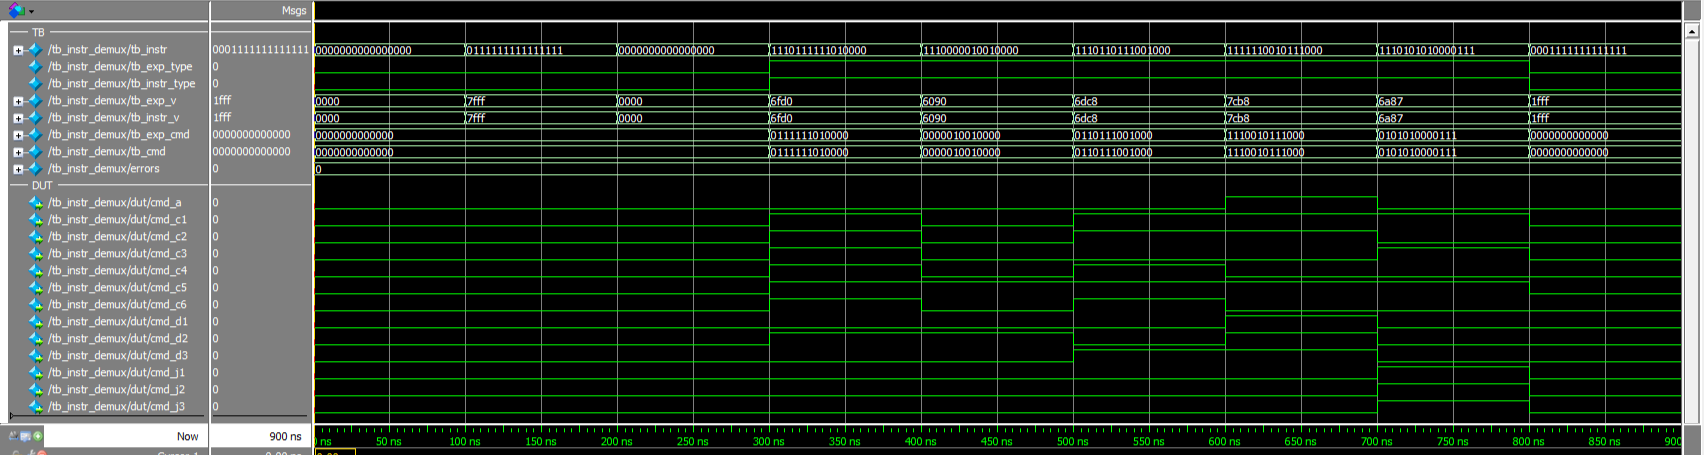
\includegraphics[width=\linewidth]{modelsim_instr_demux.png}
  \caption{Wave-Fenster \texttt{tb\_instr\_demux}.}
\end{figure}

\subsection{CPU (\texttt{tb\_cpu})}
Die Testbench erzeugt \texttt{clk50m} und \texttt{en25m} (jede zweite Flanke) und legt pro
Enable-Takt einen Befehl an. Vor der Flanke werden die kombinatorischen Ausgänge
\texttt{outM}, \texttt{writeM} und \texttt{addressM} geprüft, nach der Flanke \texttt{pc} und
die internen Register A und D. Das Programm enthält die Befehle aus Table 1 und testet
zusätzlich:
\begin{itemize}
  \item \texttt{D=M}: Mit a = 1 rechnet die ALU mit \texttt{inM}.
  \item Sprünge: \texttt{JGT}, \texttt{JEQ}, \texttt{JLT} und \texttt{JMP} werden ausgeführt,
        \texttt{JLT}, \texttt{JNE} und \texttt{JGE} jeweils mit nicht erfüllter Bedingung.
  \item \texttt{AMD=-1}: Alle drei Ziele werden gleichzeitig geschrieben. Danach ist
        A = \texttt{0xffff}, \texttt{addressM} zeigt nur die unteren 15 Bit (\texttt{0x7fff}).
  \item Überlauf des PC von \texttt{0x7fff} auf \texttt{0x0000} sowie Reset.
\end{itemize}
Bei A-Befehlen sind alle Steuerbits 0, die ALU rechnet dann \texttt{D \& A}. Dieser Wert liegt
an \texttt{outM}, wird aber wegen \texttt{writeM = 0} nicht verwendet.

\VerbatimInput[fontsize=\tiny, frame=single]{transcript_cpu.txt}

\begin{figure}[H]\centering
  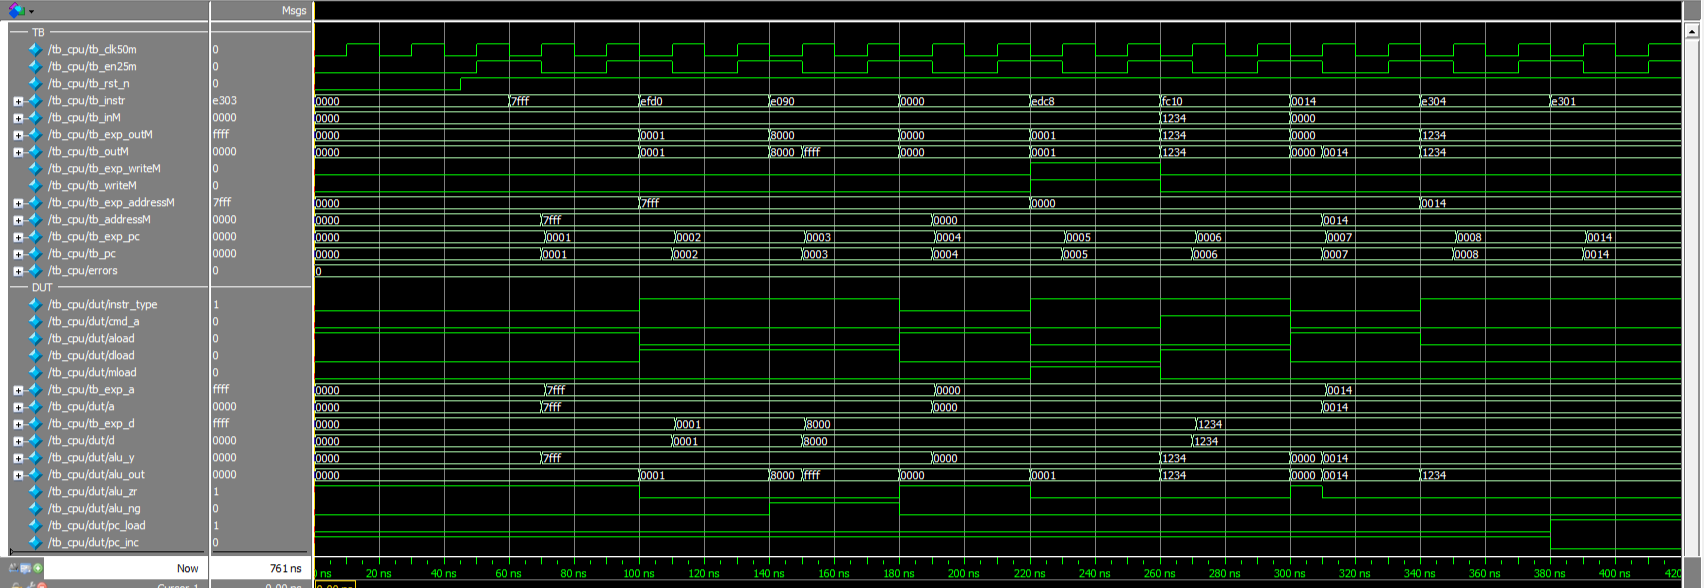
\includegraphics[width=\linewidth]{modelsim_cpu_1.png}
  \caption{Wave-Fenster \texttt{tb\_cpu}, 0--420\,ns: Befehle aus Table 1, \texttt{D=M},
  erster Sprung (\texttt{D;JGT} $\rightarrow$ pc = \texttt{0x14}).}
\end{figure}

\begin{figure}[H]\centering
  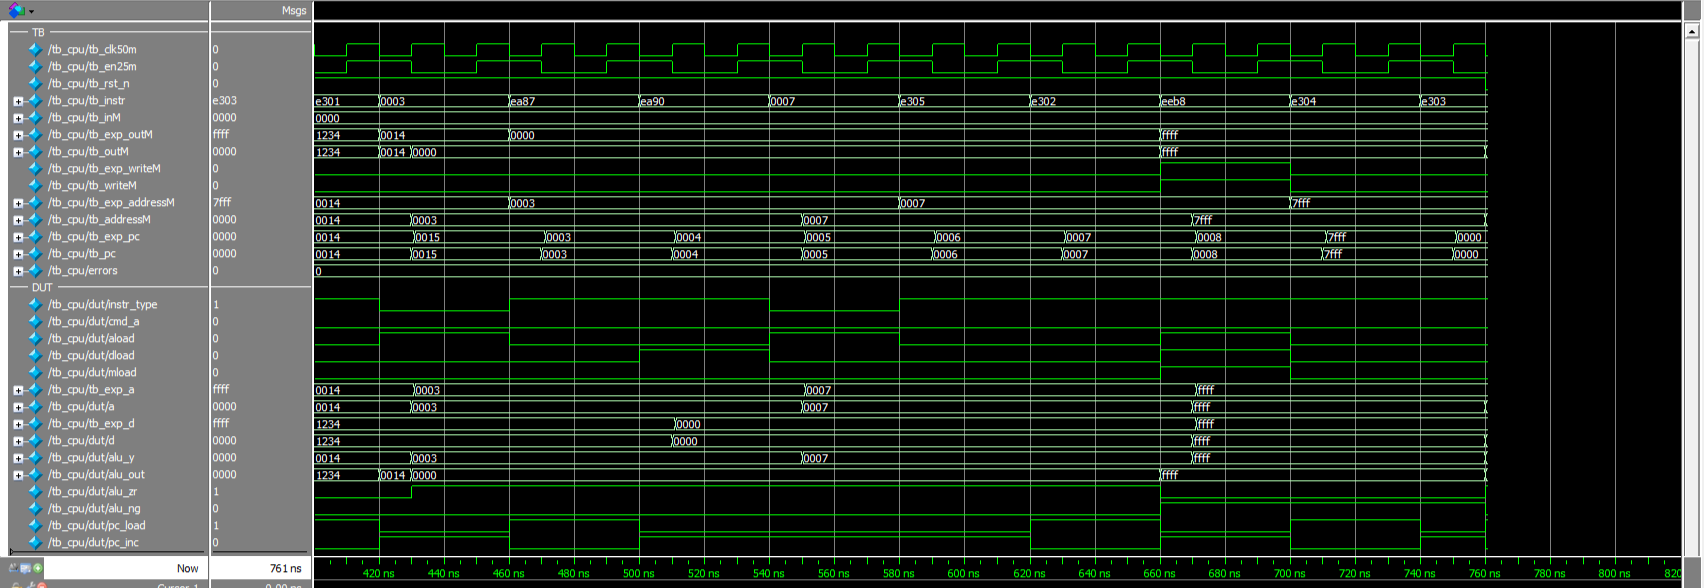
\includegraphics[width=\linewidth]{modelsim_cpu_2.png}
  \caption{Wave-Fenster \texttt{tb\_cpu}, 400--820\,ns: \texttt{0;JMP}, \texttt{JEQ},
  \texttt{AMD=-1} (\texttt{writeM = 1}), \texttt{JLT} auf \texttt{0x7fff} und Überlauf des PC.}
\end{figure}

\paragraph{Ergebnis} Beide Testbenches melden PASS, der Fehlerzähler bleibt 0. Decoder und CPU
erfüllen damit die Spezifikation.

\section{Diskussion der Implementierungsart}
\begin{tabular}{>{\raggedright}p{3.4cm}>{\raggedright}p{5.8cm}>{\raggedright\arraybackslash}p{5.8cm}}
\toprule
Methode & Vorteile & Nachteile \\ \midrule
Decoder mit \texttt{case} über alle Befehle &
Jeder Befehl steht ausgeschrieben im Code. &
28 comp-Codes $\times$ 8 dest $\times$ 8 jump -- viel zu viele Fälle, obwohl die Bits nur
durchgereicht werden. \\[2mm]
\textbf{Decoder als Bit-Zuordnung} (gewählt) &
Wenige Zeilen, direkt aus dem Befehlsformat ablesbar. &
Welche Funktion ein Bitmuster hat, sieht man nur mit der Tabelle aus der Angabe. \\[2mm]
Ganze CPU in einem Modul &
Weniger Ports und Instanzen. &
ALU, Register und PC könnten nicht einzeln getestet und wiederverwendet werden. \\[2mm]
\textbf{Strukturell aus Modulen} (gewählt) &
Entspricht dem Blockschaltbild. Die vorgegebenen Module werden unverändert
wiederverwendet. &
Viele Verbindungssignale, interne Register sind nur hierarchisch (\texttt{dut.a}) prüfbar. \\[2mm]
Eigener 25-MHz-Takt statt Enable &
Kein Enable-Signal nötig. &
Abgeleitete Takte im FPGA führen zu Skew und Timing-Problemen. Mit \texttt{en25m} bleibt alles
in einer Taktdomäne. \\
\bottomrule
\end{tabular}

\end{document}
